\subsection{Dynamic Bayesian Network Design}\label{section:dynamic-bayesian-network}

With the types of variables described, a dynamic Bayesian network, \figref{figure:dynamic-bayesian-network}, and the variables dependency herein will be explained.

\figref{figure:dynamic-bayesian-network}, is divided into timeslices, a new timeslice is created when the sensors registers a new value. 
All the variables in the dynamic Bayesian network are stochastic continuous variables.
The independent variables in the network are the \textit{Acc} and \textit{Gyro} variables, which are the information variables.
The mean values are read from the accelerometer and the gyroscope respectively. 

The \textit{Atan2} variable transforms acceleration values into angles, explained in \secref{section:gyroscope}.
The \textit{Comp}, short for Complementary Filter, variable contains angles obtained by utilising the complementary filter, which is dependent on two angles from the Gyro and Atan2 variable, explained in \secref{section:gyroscope}.
\textit{SF}, short for Sensor Fusion, serves the purpose of combining the collected data and output a corrected acceleration.
The \textit{MA}, short for Moving Average, variable takes the calculated acceleration value and applies a moving-average filter to it, as described in \secref{subsection:exponential-moving-average}.

\begin{figure}[H]
\centering
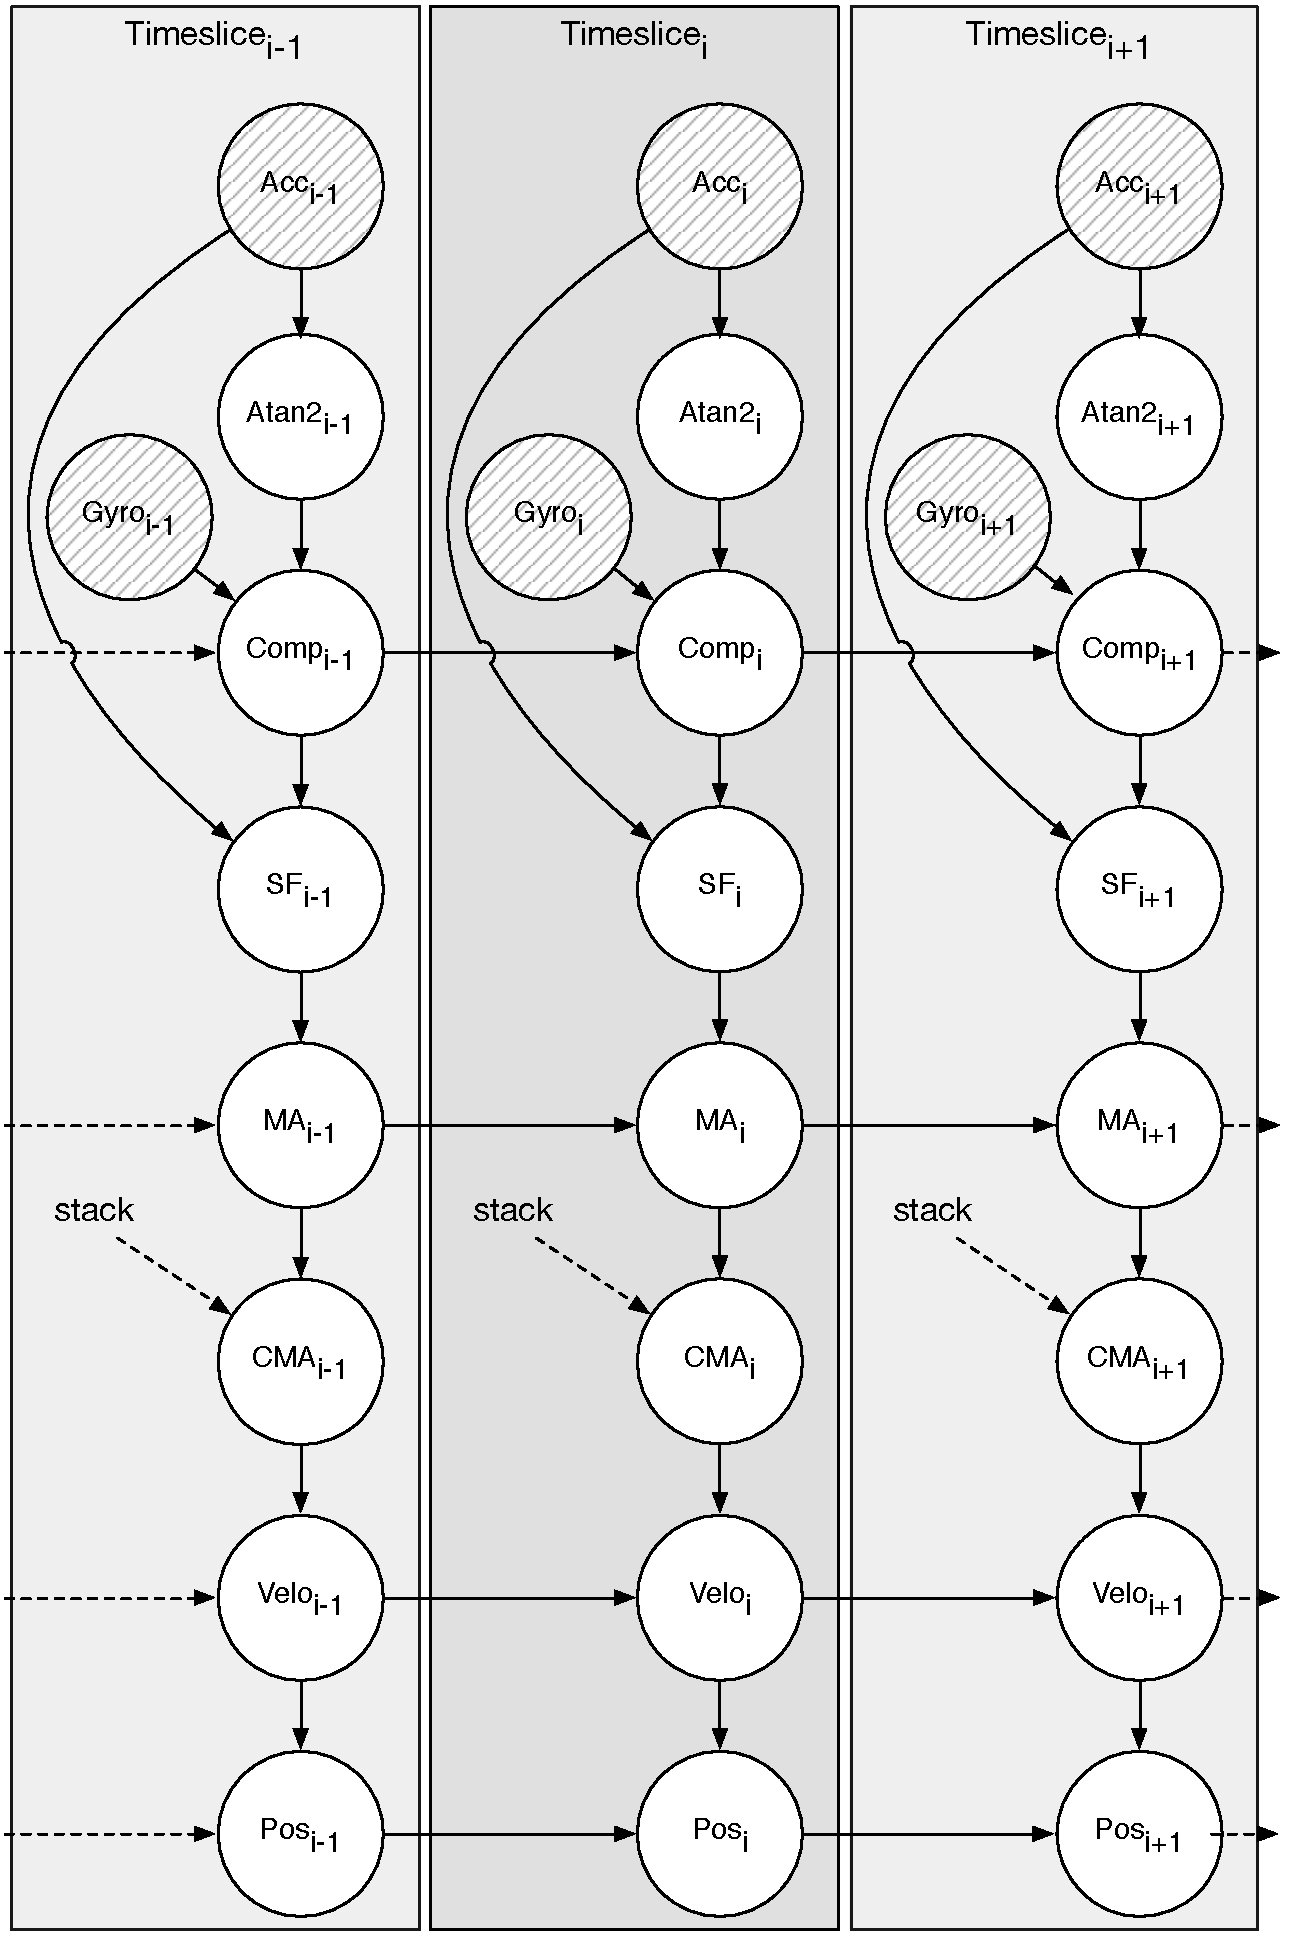
\includegraphics[scale=0.6]{media/dynamic-bayesian-network}
\caption{Dynamic Bayesian Network}
\label{figure:dynamic-bayesian-network}
\end{figure}

To make sure, every acceleration is followed by an equal deceleration, the \textit{CMA}, short for Corrected Moving Average, variable is implemented.
The purpose of CMA is to save MA variables in a stack, so that once deceleration begins, the application will pop elements from the stack and use these values negated.

The \textit{Velo} variable calculates the current velocity by using the values obtained from the CMA and previous Velo variables. 
Lastly, the \textit{Pos} variable calculates a new position, by looking at the previous Pos and the current Velo variable.

Probability distributions will be determined as described in \secref{section:normal-distribution}.
The structure of the dynamic Bayesian network is based on the physical laws for the relation between acceleration, velocity, and position, as described in \secref{sec:position-calculations}.